% 2-15-rb-tree.tex

%%%%%%%%%%%%%%%%%%%%
\documentclass[a4paper, justified]{tufte-handout}

% hw-preamble.tex

% geometry for A4 paper
% See https://tex.stackexchange.com/a/119912/23098
\geometry{
  left=20.0mm,
  top=20.0mm,
  bottom=20.0mm,
  textwidth=130mm, % main text block
  marginparsep=5.0mm, % gutter between main text block and margin notes
  marginparwidth=50.0mm % width of margin notes
}

% for colors
\usepackage{xcolor} % usage: \color{red}{text}
% predefined colors
\newcommand{\red}[1]{\textcolor{red}{#1}} % usage: \red{text}
\newcommand{\blue}[1]{\textcolor{blue}{#1}}
\newcommand{\teal}[1]{\textcolor{teal}{#1}}

\usepackage{todonotes}

% heading
\usepackage{sectsty}
\setcounter{secnumdepth}{2}
\allsectionsfont{\centering\huge\rmfamily}

% for Chinese
\usepackage{xeCJK}
\usepackage{zhnumber}
\setCJKmainfont[BoldFont=FandolSong-Bold.otf]{FandolSong-Regular.otf}

% for fonts
\usepackage{fontspec}
\newcommand{\song}{\CJKfamily{song}} 
\newcommand{\kai}{\CJKfamily{kai}} 

% To fix the ``MakeTextLowerCase'' bug:
% See https://github.com/Tufte-LaTeX/tufte-latex/issues/64#issuecomment-78572017
% Set up the spacing using fontspec features
\renewcommand\allcapsspacing[1]{{\addfontfeature{LetterSpace=15}#1}}
\renewcommand\smallcapsspacing[1]{{\addfontfeature{LetterSpace=10}#1}}

% for url
\usepackage{hyperref}
\hypersetup{colorlinks = true, 
  linkcolor = teal,
  urlcolor  = teal,
  citecolor = blue,
  anchorcolor = blue}

\newcommand{\me}[4]{
    \author{
      {\bfseries 姓名:}\underline{#1}\hspace{2em}
      {\bfseries 学号:}\underline{#2}\hspace{2em}\\[10pt]
      {\bfseries 评分:}\underline{#3\hspace{3em}}\hspace{2em}
      {\bfseries 评阅:}\underline{#4\hspace{3em}}
  }
}

% Please ALWAYS Keep This.
\newcommand{\noplagiarism}{
  \begin{center}
    \fbox{\begin{tabular}{@{}c@{}}
      请独立完成作业,不得抄袭。\\
      若得到他人帮助, 请致谢。\\
      若参考了其它资料,请给出引用。\\
      鼓励讨论,但需独立书写解题过程。
    \end{tabular}}
  \end{center}
}

\newcommand{\goal}[1]{
  \begin{center}{\fcolorbox{blue}{yellow!60}{\parbox{0.50\textwidth}{\large 
    \begin{itemize}
      \item 体会``思维的乐趣''
      \item 初步了解递归与数学归纳法 
      \item 初步接触算法概念与问题下界概念
    \end{itemize}}}}
  \end{center}
}

% Each hw consists of four parts:
\newcommand{\beginrequired}{\hspace{5em}\section{作业 (必做部分)}}
\newcommand{\beginoptional}{\section{作业 (选做部分)}}
\newcommand{\beginot}{\section{Open Topics}}
\newcommand{\begincorrection}{\section{订正}}
\newcommand{\beginfb}{\section{反馈}}

% for math
\usepackage{amsmath, mathtools, amsfonts, amssymb}
\newcommand{\set}[1]{\{#1\}}

% define theorem-like environments
\usepackage[amsmath, thmmarks]{ntheorem}

\theoremstyle{break}
\theorempreskip{2.0\topsep}
\theorembodyfont{\song}
\theoremseparator{}
\newtheorem{problem}{题目}[subsection]
\renewcommand{\theproblem}{\arabic{problem}}
\newtheorem{ot}{Open Topics}

\theorempreskip{3.0\topsep}
\theoremheaderfont{\kai\bfseries}
\theoremseparator{:}
\theorempostwork{\bigskip\hrule}
\newtheorem*{solution}{解答}
\theorempostwork{\bigskip\hrule}
\newtheorem*{revision}{订正}

\theoremstyle{plain}
\newtheorem*{cause}{错因分析}
\newtheorem*{remark}{注}

\theoremstyle{break}
\theorempostwork{\bigskip\hrule}
\theoremsymbol{\ensuremath{\Box}}
\newtheorem*{proof}{证明}

% \newcommand{\ot}{\blue{\bf [OT]}}

% for figs
\renewcommand\figurename{图}
\renewcommand\tablename{表}

% for fig without caption: #1: width/size; #2: fig file
\newcommand{\fig}[2]{
  \begin{figure}[htbp]
    \centering
    \includegraphics[#1]{#2}
  \end{figure}
}
% for fig with caption: #1: width/size; #2: fig file; #3: caption
\newcommand{\figcap}[3]{
  \begin{figure}[htbp]
    \centering
    \includegraphics[#1]{#2}
    \caption{#3}
  \end{figure}
}
% for fig with both caption and label: #1: width/size; #2: fig file; #3: caption; #4: label
\newcommand{\figcaplbl}[4]{
  \begin{figure}[htbp]
    \centering
    \includegraphics[#1]{#2}
    \caption{#3}
    \label{#4}
  \end{figure}
}
% for margin fig without caption: #1: width/size; #2: fig file
\newcommand{\mfig}[2]{
  \begin{marginfigure}
    \centering
    \includegraphics[#1]{#2}
  \end{marginfigure}
}
% for margin fig with caption: #1: width/size; #2: fig file; #3: caption
\newcommand{\mfigcap}[3]{
  \begin{marginfigure}
    \centering
    \includegraphics[#1]{#2}
    \caption{#3}
  \end{marginfigure}
}

\usepackage{fancyvrb}

% for algorithms
\usepackage[]{algorithm}
\usepackage[]{algpseudocode} % noend
% See [Adjust the indentation whithin the algorithmicx-package when a line is broken](https://tex.stackexchange.com/a/68540/23098)
\newcommand{\algparbox}[1]{\parbox[t]{\dimexpr\linewidth-\algorithmicindent}{#1\strut}}
\newcommand{\hStatex}[0]{\vspace{5pt}}
\makeatletter
\newlength{\trianglerightwidth}
\settowidth{\trianglerightwidth}{$\triangleright$~}
\algnewcommand{\LineComment}[1]{\Statex \hskip\ALG@thistlm \(\triangleright\) #1}
\algnewcommand{\LineCommentCont}[1]{\Statex \hskip\ALG@thistlm%
  \parbox[t]{\dimexpr\linewidth-\ALG@thistlm}{\hangindent=\trianglerightwidth \hangafter=1 \strut$\triangleright$ #1\strut}}
\makeatother

% for footnote/marginnote
% see https://tex.stackexchange.com/a/133265/23098
\usepackage{tikz}
\newcommand{\circled}[1]{%
  \tikz[baseline=(char.base)]
  \node [draw, circle, inner sep = 0.5pt, font = \tiny, minimum size = 8pt] (char) {#1};
}
\renewcommand\thefootnote{\protect\circled{\arabic{footnote}}} % feel free to modify this file
%%%%%%%%%%%%%%%%%%%%
\title{第4-6讲: 加密算法}
\me{朱宇博}{191220186}{}{}
\date{\zhtoday} % or like 2019年9月13日
%%%%%%%%%%%%%%%%%%%%
\begin{document}
\maketitle
%%%%%%%%%%%%%%%%%%%%
\noplagiarism % always keep this line
%%%%%%%%%%%%%%%%%%%%
\begin{abstract}
  % \begin{center}{\fcolorbox{blue}{yellow!60}{\parbox{0.65\textwidth}{\large 
  %   \begin{itemize}
  %     \item 
  %   \end{itemize}}}}
  % \end{center}
\end{abstract}
%%%%%%%%%%%%%%%%%%%%
\beginrequired

%%%%%%%%%%%%%%%
\begin{problem}[TJ 7-7(a,b)]
Encrypt each of the following rsa messages $x$ so that $x$ is divided into blocks of integers of length $2$; that is, if $x = 142528$, encode $14$, $25$, and $28$ separately.\\
(a) n = 3551, E = 629, x = 31\\
(b) n=2257,E =47,x=23
\end{problem}

\begin{solution}
(a)\\
$y=x^{E}\mod n=31^{629}\mod 3551=2791$\\
(b)\\
$y = x^{E}\mod n=23^{47}\mod 2257=769$
\end{solution}
%%%%%%%%%%%%%%%

%%%%%%%%%%%%%%%
\begin{problem}[TJ 7-9(b)]
Decrypt each of the following rsa messages y.\\
(b)\\
n=5893,D=81,y=34
\end{problem}

\begin{solution}
$x =y^D\mod n = 34^{81}\mod 5893 = 2014$
\end{solution}
%%%%%%%%%%%%%%%

%%%%%%%%%%%%%%%
\begin{problem}[TJ 7-12]
Find integers n, E, and X such that
\[
X^{E}\equiv X \pmod n
\]
Is this a potential problem in the rsa cryptosystem?
\end{problem}

\begin{solution}
对于任意$X$,令$E=k\phi(n) + 1$,其中$k\in \mathbb{N}$,即可满足该等式。\\
这是一个potential problem in rsa。该方程说明,在给定$n$和$X$下,只需将$X$做$E$次乘法,即可获取$X$。\\
这可以看成一个加密-解密的过程。我们需要找到一组对应关系,使得$ab=E$,则有加密$y=x^{a}$, 解密$x=y^{b}$。
\end{solution}
%%%%%%%%%%%%%%%

%%%%%%%%%%%%%%%
\begin{problem}[TC 31.7-1]
Consider an RSA key set with p=11,q=29,n=319, and e=3. What value of d should be used in the secret key? What is the encryption of the message M=100?
\end{problem}

\begin{solution}
$m=\phi(pq)=(p - 1)(q-1)=280$, $ed\equiv 1\pmod{280}$. So $d$ could be $187$.\\
$y = M^{d} \mod n= 100^{3}\mod 319 =254$
\end{solution}
%%%%%%%%%%%%%%%

%%%%%%%%%%%%%%%
\begin{problem}[TC 31.7-2]
 \begin{figure}[htbp]
    \centering
    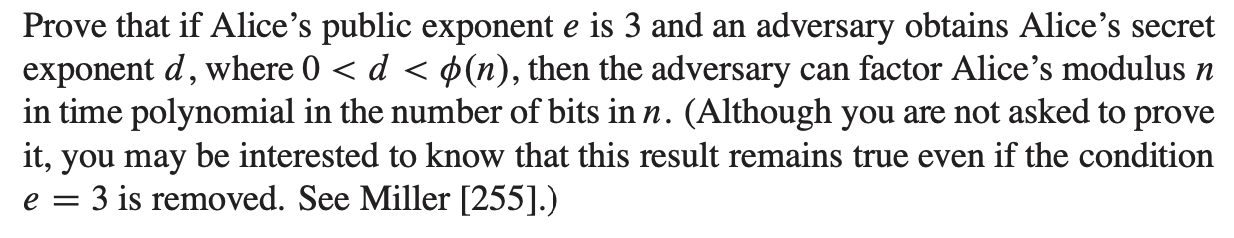
\includegraphics[width = 0.90\linewidth]{figs/a}
  \end{figure}
\end{problem}

\begin{solution}
当$n\geq 16$时,
\[
\phi(n)=(p-1)(q-1)=(p-1)(\frac{n}{p}-1)=n - (p + \frac{n}{p}) + 1 \geq n - 2\sqrt{n} + 1\geq \frac{n}{2}
\]
则有
\[
k \phi(n) = 3d-1 \leq 3n\to k \leq 6
\]
所以在$[1,6]$之间枚举整数k,即可使等式成立,求得$\phi(n)$。\\
又有$\phi(n)=(p-1)(q-1)=n - (p + \frac{n}{p}) + 1, q = \frac{n}{p}$,即可求得$p,q$。\\
因为上述计算经过常数次长度不超过$|n|$的加减乘除即可完成,故在$|n|$的多项式时间内可对$n$进行质因数分解。\\
若$n\leq 16$,则显然可在$|n|$的多项式时间内可对$n$进行质因数分解。\\
综上,得证。
\end{solution}
%%%%%%%%%%%%%%%

%%%%%%%%%%%%%%%
\begin{problem}[TC Problem 31-3]
\end{problem}

\begin{solution}
(a)\\
在该情况下,有
\[
T_n =T(n-1)+T(n-2)+O(1)
\]
解得$T(n)=O(\phi^n)$,其中$\phi=\frac{\sqrt{5}+1}{2}$\\
(b)\\
在(a)的递归基础上,运用记忆化搜索,将每个计算出的$F_i$存下,避免重复计算。则在这种情况下,每个$F_i$都只会被计算一次,且计算时间为常数,故用时为$O(n)$\\
(c)\\
根据斐波那契数列的性质,有
 $$\begin{pmatrix}F_{n+1}\\
			   F_{n}
     \end{pmatrix}
     =
     \begin{pmatrix} 
     			     1&1\\
			     1&0
     \end{pmatrix}
     \cdot
     \begin{pmatrix}F_{n}\\
     			   F_{n-1}
     \end{pmatrix}$$
 利用矩阵快速幂,即可在$O(\lg n)$时间内完成。\\
 (d)\\
 第一种:\\
 在该情况下,有
\[
\begin{aligned}
T(n) =&T(n-1)+T(n-2)+O(\lg F_{n-1})\\
=&T(n-1)+T(n-2)+O(n)
\end{aligned}
\]
解得$T(n)=O(\phi^n)$\\

\noindent 第二种:\\
计算$F_{n}$时加法操作耗时$O(n)$,则$F_n$~$F_1$中每个数被计算一次,耗时可近似为$O(n^2)$\\
故此时时间复杂度为$O(n^2)$\\

\noindent 第三种:
在该情况下,有
\[
\begin{aligned}
T(n) =&2T(n/2)+O((\lg F_{\frac{n}{2}})^2)\\
=&2T(n/2)+O(n^2)
\end{aligned}
\]
解得$T(n)=O(n^2)$\\
\end{solution}
%%%%%%%%%%%%%%%

%%%%%%%%%%%%%%%%%%%%
\beginoptional

%%%%%%%%%%%%%%%
\begin{problem}[TC Problem 31-4]
\end{problem}

\begin{solution}
\end{solution}
%%%%%%%%%%%%%%%


%%%%%%%%%%%%%%%%%%%%
\beginot
%%%%%%%%%%%%%%%
\begin{ot}[中国剩余定理]	
	向同学介绍中国剩余定理及其应用。
\end{ot}

% \begin{solution}
% \end{solution}
%%%%%%%%%%%%%%%

%%%%%%%%%%%%%%%
\begin{ot}[椭圆曲线加密(Elliptic Curve Cryptography, ECC)]	
	椭圆曲线加密是基于椭圆曲线数学理论实现的一种非对称加密算法。相比RSA,ECC优势是可以使用更短的密钥,来实现与RSA相当或更高的安全。
	
	(参考资料-1:\href{https://medium.com/dev-genius/introduction-to-elliptic-curve-cryptography-567e47b0e49e}{https://medium.com/dev-genius/introduction-to-elliptic-curve-cryptography-567e47b0e49e})
	(参考资料-2:\href{https://en.wikipedia.org/wiki/Elliptic-curve_cryptography}{https://en.wikipedia.org/wiki/Elliptic-curve\_cryptography})
	(参考资料-3:\href{https://www.jianshu.com/p/e41bc1eb1d81}{https://www.jianshu.com/p/e41bc1eb1d81})
\end{ot}


% \begin{solution}
% \end{solution}
%%%%%%%%%%%%%%%


% \vspace{0.50cm}
%%%%%%%%%%%%%%%
% \begin{ot}[]
% 
%   \noindent 参考资料:
%   \begin{itemize}
%     \item 
%   \end{itemize}
% \end{ot}

% \begin{solution}
% \end{solution}
%%%%%%%%%%%%%%%

%%%%%%%%%%%%%%%%%%%%
% 如果没有需要订正的题目,可以把这部分删掉

% \begincorrection
%%%%%%%%%%%%%%%%%%%%

%%%%%%%%%%%%%%%%%%%%
% 如果没有反馈,可以把这部分删掉
\beginfb

% 你可以写
% ~\footnote{优先推荐 \href{problemoverflow.top}{ProblemOverflow}}:
% \begin{itemize}
%   \item 对课程及教师的建议与意见
%   \item 教材中不理解的内容
%   \item 希望深入了解的内容
%   \item $\cdots$
% \end{itemize}
%%%%%%%%%%%%%%%%%%%%
% \bibliography{2-5-solving-recurrence}
% \bibliographystyle{plainnat}
%%%%%%%%%%%%%%%%%%%%
\end{document}